\documentclass{article}
\usepackage[utf8]{inputenc}
\usepackage{kotex}
\usepackage{verbatim}
\usepackage{graphicx}
\usepackage{indentfirst}
\usepackage{subfigure}
\usepackage{listings}
\usepackage{xcolor}
\usepackage{tikz}
\usetikzlibrary{graphdrawing.trees}
\usepackage{geometry}
\usepackage{amsmath}
\usepackage{amssymb}
\usepackage{enumitem}
\usepackage{verbatim}

\renewcommand{\figurename}{그림}
\renewcommand{\tablename}{표}
\renewcommand{\contentsname}{목차}
\renewcommand{\lstlistingname}{코드}
\renewcommand{\listfigurename}{\figurename 목차}
\renewcommand{\listtablename}{\tablename 목차}
\renewcommand{\lstlistlistingname}{\lstlistingname 목차}

\geometry{
    a4paper,
    left=30mm,
    right=30mm,
    top=30mm,
    bottom=40mm
}

\lstset{language=C++,
            basicstyle=\ttfamily,
            keywordstyle=\color{blue}\ttfamily,
            stringstyle=\color{red}\ttfamily,
            commentstyle=\color{teal}\ttfamily,
            numberstyle=\tiny\color{gray}\ttfamily,
            morecomment=[l][\color{magenta}]{\#}
            breakatwhitespace=false,         
            breaklines=true,                 
            captionpos=b,                    
            keepspaces=true,                 
            numbers=left,                    
            numbersep=5pt,                  
            showspaces=false,                
            showstringspaces=false,
            showtabs=false,                  
            tabsize=2
}

\title{자료구조 HW11 정렬 알고리즘 성능 비교}
\author{C211123 이준선}
\date{2022년 12월 9일}

\begin{document}

\maketitle
\tableofcontents
\listoffigures
\lstlistoflistings

\section{개요}
삽입 정렬(Insertion sort), 힙 정렬(Heap sort), 퀵 정렬(Quick sort), 자연 합병 정렬(Natural Merge Sort) 4개의 정렬 알고리즘을 구현하고, 각각의 연산 시간을 측정해 성능을 비교하였다. 테스트 파일의 종류는 크게 4가지로 다음과 같다.
\begin{enumerate}
    \item decreasing\_t : 감소하는 순서로 정렬된 데이터
    \item sorted\_t : 완전 정렬된 데이터
    \item partially\_sorted\_t : 부분적으로 정렬된 데이터
    \item random\_t : 랜덤한 순서로 섞인 데이터
\end{enumerate}

각 종류의 데이터 폴더에는 t=50부터 t=100000 까지의 15개의 테스트 파일들이 담겨 있어 총 60개의 테스트 파일이 존재한다. 한편 시간의 측정 방식은, 동일한 파일에 대해 5번 정렬을 반복하여 나온 평균 시간을 그 테스트 파일에 대한 정렬 시간으로 한다. 한편 표본이 30개 이상이면 모평균을 추정하기에 충분히 많은 표본을 확보했다고 볼 수 있다\footnote{중심극한정리}. 테스트 파일의 수가 60개이므로 충분한 표본을 확보했다고 볼 수 있기에, 별도의 데이터 첨가(augmentation)은 진행하지 않았다. 한편 main 함수의 경우, 실습 조교님께서 직접 올려주신 코드를 그대로 사용하되, 5번 반복해 평균 시간을 구할 수 있도록 일부만 부분 수정하였다. 정렬 알고리즘의 경우 교재와 강의록에 알고리즘과 코드가 포함되었을 경우 최대한 이를 반영하였다.

한편 본 보고서에서 `성능이 높다(좋다)'라는 말은 시간 복잡도가 낮다는 의미이며, 이는 정렬을 수행하는데 필요한 연산 시간이 더 짧게 걸린다는 의미이다. `성능이 낮다(좋지 않다)'라는 뜻은 그 반대이다.

\section{삽입 정렬(Insertion sort)}
\subsection{삽입 정렬 코드}
\begin{lstlisting} [language=C++, escapeinside=``, caption=insertion sort, label={lstlinsting:insertion sort}]
template <class T>
void Insert(const T& e, T* list, int i)
{
	// e`를 정렬된 리스트` list[1:i]`에 삽입하여`
	// `결과 리스트` list[1:i+1]`도 정렬되게 한다.`
	// `배열` list`는 적어도` i+2 `원소를 포함할 공간을 갖고 있어야 한다.`
	list[0] = e;
	while (e < list[i]) {
		list[i + 1] = list[i];
		i--;
	}
	list[i + 1] = e;
}

template <class T>
void insertion_sort(T* list, int n)
{
	// list[1:n]`을 삽입 정렬로 정렬한다.`
	for (int i = 2; i <= n; i++)
		Insert(list[i], list, i - 1);
}
\end{lstlisting}

\subsection{삽입 정렬 설명}
\begin{figure} [h]
    \centering
    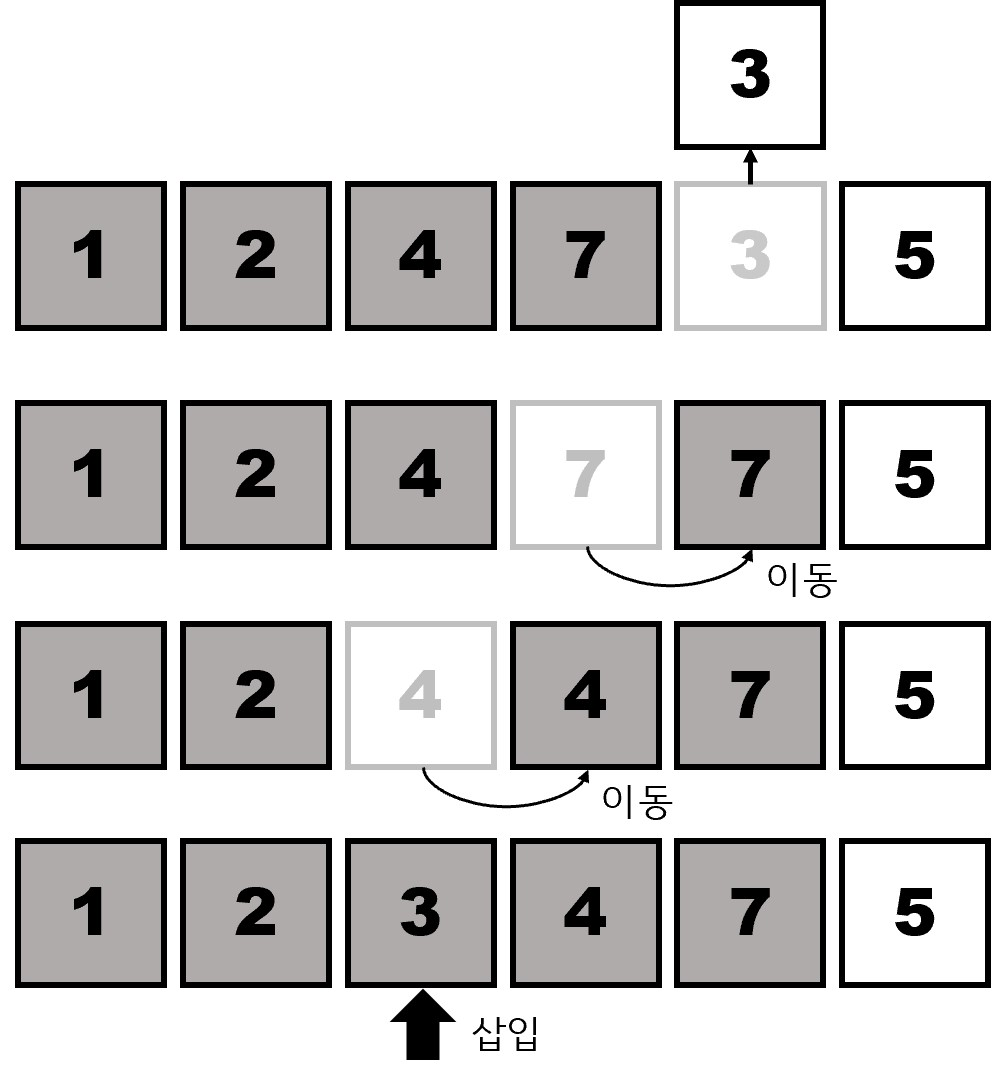
\includegraphics[width=0.4\textwidth]{insertion_sort_process.jpg}
    \caption{삽입 정렬 과정}
    \label{fig:insetion sort process}
\end{figure}

삽입 정렬은 데이터의 모든 요소를 앞에서부터 차례대로 이미 정렬된 배열 부분과 비교하여, 자신의 위치를 찾아 삽입함으로써 정렬을 완성하는 알고리즘이며, 최악의 경우 $O(n^2)$의 시간복잡도를 갖는 알고리즘이다. 그러나 $O(n^2)$의 시간 복잡도를 갖는 다른 알고리즘들-버블 정렬이나 선택 정렬 등에 비해 근소하게 효율적이라고 알려져 있다. 특히 최선의 경우 시간 복잡도가 $O(n)$으로, 최선의 경우에도 $O(n^2)$의 시간 복잡도를 갖는 선택 정렬 등과 비교했을 시 우위를 가지고 있다.

한편 삽입 정렬, 버블 정렬, 선택 정렬과 같은 단순하지만 비효율적인 알고리즘들은 코드가 단순해 구현이 매우 쉽고, 함수 호출로 인한 오버헤드가 발생하지 않기 때문에\footnote{오버헤드가 발생하지 않기 때문에, 실제로 데이터 수가 50개, 100개인 경우 오히려 삽입 정렬의 성능이 다른 $O(n\log{n})$인 알고리즘보다 높은 성능을 보여주었다.} 데이터 수가 약 100개 미만으로 적은 경우 자주 사용한다.

삽입 정렬의 자세한 과정은 그림 \ref{fig:insetion sort process}에서 확인할 수 있다. 그림 \ref{fig:insetion sort process}와 같이 초기 상태인 \{1, 2, 4, 7, 3, 5\}에서, 3을 정렬한다고 가정하자. 이때 삽입 정렬은 왼쪽부터 순차적으로 정렬하기에, 정렬 대상의 앞은 이미 정렬된 상태임이 보장된다. 즉 정렬 대상인 3 앞은 \{1, 2, 4, 7\}의 상태로 이미 정렬되어 있다. 3을 떼어내서, 3보다 작거나 같은 숫자가 나오기 전까지 앞의 숫자와 차례대로 비교하며 한 칸씩 뒤로 민다. 그러다 3보다 작은 숫자인 2를 만나면, 뒤로 당기는 반복문을 종료한 후 그 자리에 3을 삽입한다.

n개의 데이터가 있을 때, 최악의 경우 $\sum\limits_{i=1}^{n-1}i=1+2+\cdots+(n-1)=\cfrac{n(n-1)}{2}$번의 비교를 수행한다. 따라서 최악의 시간복잡도는 앞에서 언급한 대로 $O(n^2)$이다.

코드 \ref{lstlinsting:insertion sort}은 삽입 정렬을 구현한 코드이다. 코드는 교재를 일부 참고하였다.

\section{힙 정렬(Heap sort)}
\subsection{힙 정렬 코드}
\begin{lstlisting} [language=C++, escapeinside=``, caption=heap sort, label={lstlinsting:heap sort}]
// heap sort
template <class T>
void Adjust(T* list, const int root, const int n)
{
	// root`를 루트 노드로 하는 이진 트리가 힙 성질을 만족하도록 조정`
	// root`의 왼쪽과 오른쪽 서브트리는 이미 힙 성질을 만족하고 있다. 노드 인덱스는 n보다 크지 않다.`
	T e = list[root];
	// e`에 대한 적절한 위치를 탐색`
	int j = root * 2;
	for (; j <= n; j *= 2) {
		if (j < n && list[j] < list[j + 1]) j++;
		if (e >= list[j]) break;
		list[j / 2] = list[j];
	}
	list[j / 2] = e;
}

template <class T>
void heap_sort(T* list, const int n)
{
	// list[1:n]`을 비감소 순으로 정렬한다.`
	for (int i = n / 2; i >= 1; i--) // `힙로 조정`
		Adjust(list, i, n);
	
	for (int i = n - 1; i >= 1; i--) { // sort
		swap(list[1], list[i + 1]); // `현 힙의 처음과 마지막을 교환`
		Adjust(list, 1, i); // `힙로 조정`
	}
}
\end{lstlisting}
\subsection{힙 정렬 설명}
\begin{figure}
    \centering
    \begin{tikzpicture}[nodes={draw, circle}]
    \node{1}
    child { node {4} 
        child { node {7} 
            child { node {35} }
            child { node {27}}
        }
        child { node {9} }
        child [missing]
    }
    child { node {8} 
        child [missing]
        child { node {11} }
        child { node {25} }
    };
 
\end{tikzpicture}
    \caption{Heap}
    \label{fig:heap structure}
\end{figure}

힙 정렬은 자료구조 힙을 활용하여 정렬을 하는 알고리즘이다. 힙은 이진완전트리로써, 우선 순위가 높은 원소가 서브 트리의 루트 노드에 위치하는 자료구조이다. 그림 \ref{fig:heap structure}은 숫자가 작을 수록 우선 순위가 높게 설정된 최소 힙이다. 단순히 모든 데이터를 힙에 전부 넣었다 다시 빼내는 것만으로 정렬이 완성된다. 이때 n개의 데이터에 대해 최소 힙을 구성하는 시간은 $O(\log{n})$이다\footnote{힙의 높이가 $\log_2{n}$이고, $\log_2{n}=\cfrac{\log{n}}{\log{2}}$에서 $\log{2}$는 상수이므로 $O(\log{n})$ 꼴로 나타낼 수 있다.}. 이를 데이터 n개만큼 반복해서 push, pop 과정이 이루어지므로 시간 복잡도는 $O(n\log{n})$이 된다.

코드 \ref{lstlinsting:heap sort}는 힙 정렬 알고리즘을 보여준다. 교재를 일부 참고하였다. 함수 Adjust는 힙를 만드는 함수이다. Adjust를 반복적으로 호출하여 최대 힙를 만든다. 그런 다음에, 힙의 첫 번째 레코드와 마지막 레코드를 교환한다. 첫 번째 레코드는 최대 키를 가지므로 이 교환을 통해 최대 키를 가진 레코드를 정렬된 배열의 정확한 위치로 들어가게 한다. 그런 다음에는 힙의 크기를 줄인 후 다시 힙를 조정한다. 이 교환, 힙 크기 축소, 힙 재조정 과정을 n-1번 반복하면 배열 list[1:n] 전체를 정렬하게 된다.

\subsection{힙 정렬 시간복잡도}
Assume that $2k^{-1}\leq n \leq 2^k$ for $k$ level of tree, and $n$ elements, then number of \textit{i}-th level node is $2^{i-1}$. At the first \textbf{for} loop, heap\_sort function calls the Adjust function once for each node with a child. Thus time consumed for this loop equals for each level, number of nodes for that level multiplies max distance which each node can move. This value shall not exceed the following values on equation \ref{eq:eq heap}
\begin{equation}
\label{eq:eq heap}
\begin{aligned}
    \sum\limits_{1\leq i \leq k}{2^{i-1}(k-1)} 
    = \sum\limits_{1\leq i \leq k-1}{2^{k-i-1}i} 
    \leq n = \sum\limits_{1\leq i \leq k-1}{\cfrac{1}{2^i}} < 2n = O(n)
\end{aligned}
\end{equation}

\section{퀵 정렬(Quick Sort)}
\subsection{퀵 정렬 코드}
\begin{lstlisting} [language=C++, escapeinside=``, caption=quick sort, label={lstlinsting:quick sort}]

// `입력된 세 개의 인수 중 중앙값(median)에 해당하는 index를 반환`
template <class T>
int medianIdx(T* list, int a, int b, int c)
{
	if (list[a] < list[b]) {
		if (list[b] < list[c]) return b;
		else if (list[a] < list[c]) return c;
		else return a;
	}
	else {
		if (list[a] < list[c]) return a;
		else if (list[b] < list[c]) return c;
		else return b;
	}
}

// quick sort
template <class T>
void quick_sort(T* list, const int left, const int right)
{
	if (left < right) {
		int low = left, high = right + 1;
		// `현재 서브리스트에 있는 첫 번째, 중앙, 마지막 키 중에서 메디안을 선택`
		int pivotIdx = medianIdx(list, left, (left + right) / 2, right);
		
		// `이렇게 스왑해주면 교재에서 사용한 기존 코드가 그대로 유지된다.`
		swap(list[left], list[pivotIdx]);
		
		T pivot = list[left];
		do {
			do low++; while (list[low] < pivot);
			do high--; while (list[high] > pivot);
			if (low < high) swap(list[low], list[high]);
		} while (low < high);
		swap(list[left], list[high]); // `피벗을 기준선 위치로 이동한다.`

		quick_sort(list, left, high - 1);
		quick_sort(list, high + 1, right);
	}
}
\end{lstlisting}
\subsection{퀵 정렬 설명}
\begin{figure}
    \centering
    \subfigure[퀵 정렬 과정 1]{
        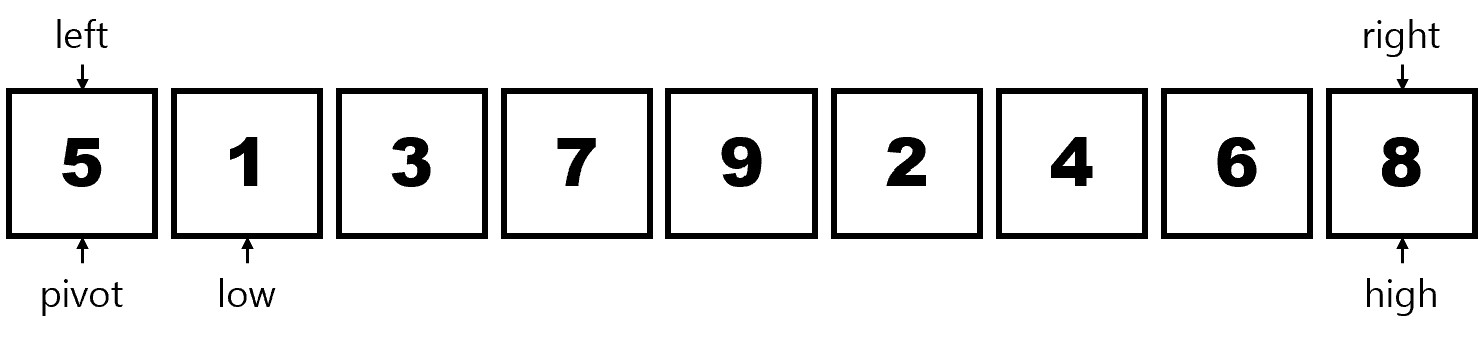
\includegraphics[width=\textwidth]{quicksort_a.jpg}
        \label{fig:quicksort_a}
    }
    \subfigure[퀵 정렬 과정 2]{
        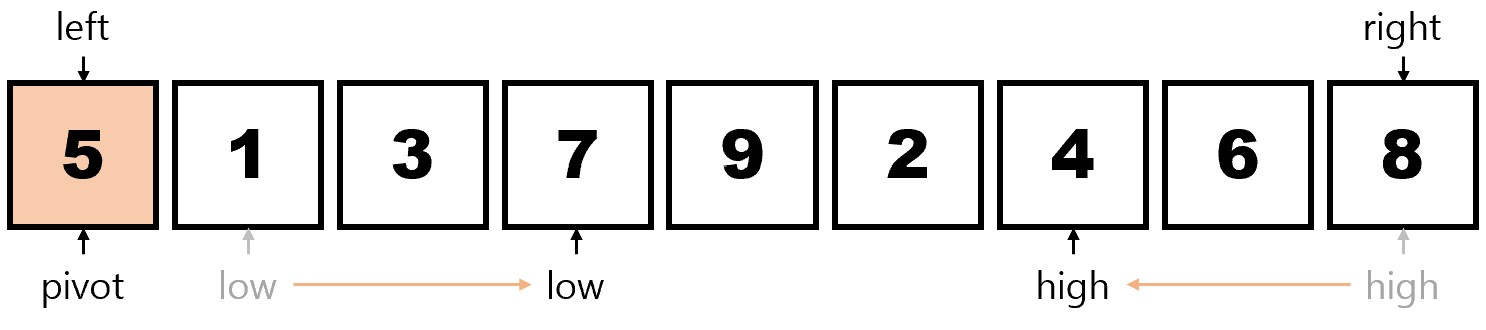
\includegraphics[width=\textwidth]{quicksort_b.jpg}
        \label{fig:quicksort_b}
    }
    \subfigure[퀵 정렬 과정 3]{
        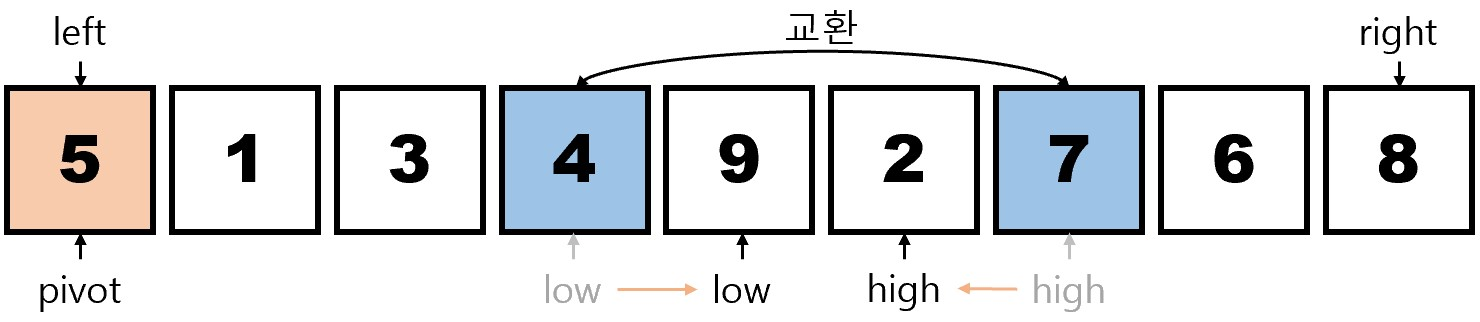
\includegraphics[width=\textwidth]{quicksort_c.jpg}
        \label{fig:quicksort_c}
    }
    \subfigure[퀵 정렬 과정 4]{
        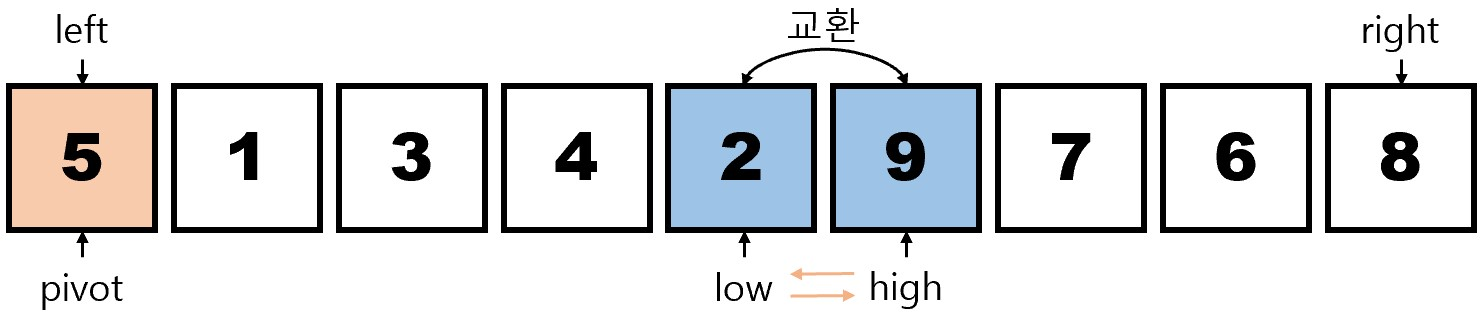
\includegraphics[width=\textwidth]{quicksort_d.jpg}
        \label{fig:quicksort_d}
    }
    \subfigure[퀵 정렬 과정 5]{
        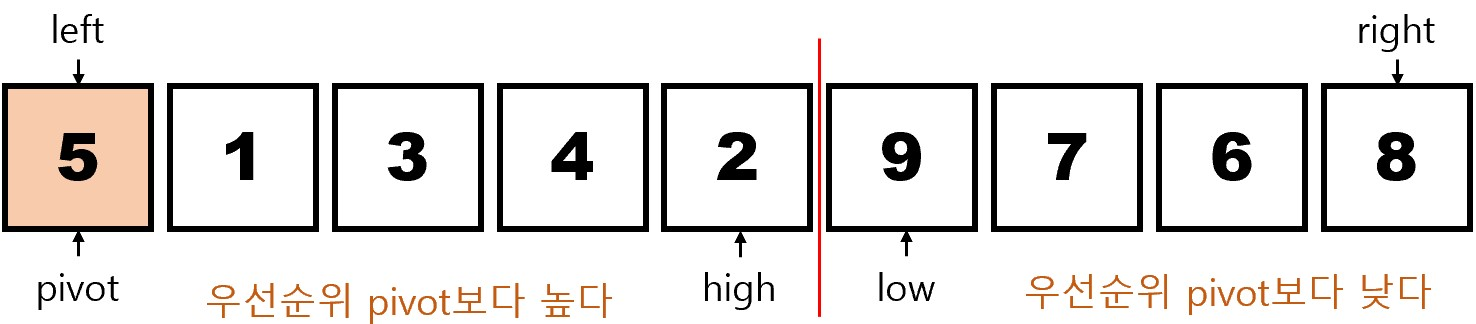
\includegraphics[width=\textwidth]{quicksort_e.jpg}
        \label{fig:quicksort_e}
    }
    \caption{퀵 정렬 과정}
    \label{fig:quicksort}
\end{figure}
퀵 정렬은 일반적으로 알려진 정렬 방법 중 가장 좋은 평균 성능을 가지고 있다. 비록 최악의 경우 시간 복잡도는 $O(n^2)$이지만, 평균 시간 복잡도는 $O(n\log{n})$이다. 그러나 알려진 $O(n\log{n})$의 시간 복잡도를 갖는 다른 알고리즘에 비해 퀵 정렬은 더 우수한 성능을 가진다고 알려져 있다. C++ STL의 sort 알고리즘도 일반적으로 퀵 정렬을 활용한다.

퀵 정렬에서는 정렬할 레코드 중에서 피벗(pivot)을 선택한다. 다음에는 정렬할 레코드들을 다시 정돈해서 피벗의 왼쪽에는 레코드 키들이 피벗의 키보다 작거나 같고, 피벗의 오른쪽에는 레코드 키들이 피벗의 키보다 크거나 같게 되도록 한다.

퀵 정렬에서 사용하는 변수는 다음과 같다:
\begin{itemize}
    \item left: 정렬 대상의 가장 왼쪽 원소
    \item right: 정렬 대상의 가장 오른쪽 원소
    \item pivot: 피벗, 중심점, 중심축
    \item low: 피벗을 제외한 가장 왼쪽 지점
    \item high: 피벗을 제외한 가장 오른쪽 지점
\end{itemize}

퀵 정렬의 자세한 과정은 다음과 같다(그림 \ref{fig:quicksort} 참조):
\begin{enumerate}
    \item 그림 \ref{fig:quicksort_a}: 초기 상태
    \item 그림 \ref{fig:quicksort_b}: low, high를 이동한다. 이때 이동 조건은 각각 다음과 같다.
    \begin{itemize}
        \item low의 오른쪽 방향 이동 : pivot보다 정렬 우선 순위가 낮은 원소를 만날 때까지
        \item high의 왼쪽 방향 이동 : pivot보다 정렬 우선 순위가 높은 원소를 만날 때까지
    \end{itemize}
    위 이동 조건에 따라 low는 7, high는 4를 가리키게 된다.
    \item 그림 \ref{fig:quicksort_c}: low와 high를 교환한다. low와 high는 교환 후 다시 이동한다.
    \item 그림 \ref{fig:quicksort_d}: low와 high가 2와 9를 교환한 이후, 다시 이동하면 low와 high의 역전\footnote{low와 high의 상대 위치가 역전되는 현상. 즉 $\text{low} < \text{high}$의 관계에서 $\text{low} > \text{high}$의 관계로 바뀌게 되는 현상.}이 일어난다.
    \item 그림 \ref{fig:quicksort_e}: high와 low 사이에 기준선이 생긴다. 이때 high, low의 이동, 교환 과정을 거치며 pivot보다 정렬 우선 순위가 높은 원소들은 기준선의 왼쪽으로, 높은 원소들은 기준선의 오른쪽으로 이동된 상태이다. 그 결과로 기준선의 왼쪽은 pivot보다 우선순위가 높은 것이 확정되며, 기준선의 오른쪽은 pivot보다 우선순위가 낮은 것이 확정된다. pivot의 위치는 기준선의 위치이다.
    \item 위 과정을 재귀 함수를 통해 반복한다.
\end{enumerate}

코드 \ref{lstlinsting:quick sort}에서는 위 과정이 구현되어 있다. 구현 시 교재를 일부 참조하였다. 한편 위 코드에서 주목해야 할 점은 pivot의 선택 기준인데, 그림 \ref{fig:quicksort}과 위 과정에서는 pivot을 단순히 정렬 대상의 가장 왼쪽 원소로 삼았다. 그러나 교재에서 언급된 대로, 퀵 정렬의 최악의 시간 복잡도를 갖는 상황을 줄이기 위해선 pivot의 선택 방식을 중앙값(median, 메디안)으로 선택해야 할 필요가 있다. 이 경우 최악의 경우를 만날 가능성이 비약적으로 줄어들면서, 퀵 정렬의 성능이 상승한다. 즉 $\text{pivot} = \text{median}\{K_{left}, K_{\frac{left+right}{2}}, K_{right}\}$이다. 코드 \ref{lstlinsting:quick sort}에서 medianIdx 함수를 통해 중앙값의 인덱스를 구하고, 이 인덱스 원소를 left와 교환하였다. 이후는 교재의 방식과 동일하다.

\subsection{퀵 정렬 시간복잡도}
Let $T_{avg}(n)$ be the expected time for function quick\_sort to sort a list with n records. Then $\exists k \text{ s.t. } T_{avg}(n)\leq kn\ln n \text{ for } n \geq 2$ which implies time complexity of quick sort algorithm is $O(n\log n)$

\textbf{Prove:} In the call to quick\_sort(list, 1, n), the pivot gets placed at position j. This leaves us with the problem of sorting two sublists of size j-1 and n-j. The expected time for this is $T_{avg}(j-1)+T_{avg}(n-j)$. The remainder of the function clearly takes at most $cn$ time for some constant $c$. Since $j$ may take on any vlaues 1 to $n$ with equal probability, we have equation \ref{eq:eq1} for $n\geq 2$.
\begin{equation}
\label{eq:eq1}
T_{avg}(n)\leq cn + \cfrac{1}{n}\sum\limits_{j=1}^{n}{(T_{avg}(j-1)+T_{avg}(n-j))} = cn+\cfrac{2}{n}\sum\limits_{j=0}^{n-1}{T_{avg}(j)}
\end{equation}
We may assume that for $\forall b \in \mathbb{R}$, $T_{avg}(0)\leq b \text{ and } T_{avg}(1)\leq b$ so that $T_{avg}(0)+T_{avg}(1)\leq 2b$. We shall now show that $T_{avg}(n)\leq kn\ln n \text{ for } n\geq 2$ and $k=2(b+c)$. The proof is by induction on n.
\begin{itemize}
    \item Induction base: For $n=2$, equation \ref{eq:eq1} yields $T_{avg}(2) \leq 2c + T_{avg}(0)+T_{avg}(1) \leq 2c + 2b \leq \overbrace{kn\ln 2}^{\because 1 < 2\ln 2}$
    \item Induction hypothesis: $T_{avg}(n)\leq kn\ln n$ for $1\leq n < m$
    \item Induction Step: From equation \ref{eq:eq1} and the induction hypothesis we have equation \ref{eq:eq2}
    \begin{equation}
    \label{eq:eq2}
        T_{avg}(m) \leq cm + \cfrac{4b}{m}+\cfrac{2}{m}\sum\limits_{j=2}^{m-1}{T_{avg}(j)} \leq cm+\cfrac{4b}{m}+\cfrac{2k}{m}\sum\limits_{j=2}^{m-1}{j\ln j}
    \end{equation}
    Since $j\ln j$ is an increasing function of $j$, equation \ref{eq:eq2} yields equation \ref{eq:eq3}
\begin{equation}
\label{eq:eq3}
\begin{aligned}
    T_{avg}(m) & \leq cm+\cfrac{4b}{m}+\cfrac{2k}{m}\int_{2}^{m} x\ln x \,dx \\
            & = cm+\cfrac{4b}{m}+\cfrac{2k}{m}\overbrace{(\cfrac{m^2\ln m}{2}-\cfrac{m^2}{4})}^\text{use partial integral} \\
            & = cm + \cfrac{4b}{m}+km\ln m - \cfrac{km}{2} \\
            & \leq km\ln {m} \text{, for } m\geq 2 \blacksquare
\end{aligned}
\end{equation}
\end{itemize}


\section{자연 합병 정렬(Natural merge sort)}
\subsection{자연 합병 정렬 코드}
\begin{lstlisting} [language=C++, escapeinside=``, caption=natural merge sort, label={lstlinsting:natural merge sort}]
// natural_merge_sort
template <class T>
void Merge(T* initList, T* mergedList, const int l, const int m, const int n)
{
	// initList[l:m]`과 `initList[m+1:n]`는 정렬된 리스트`
	// `이들은 정렬된 리스트 mergedList[l:n]로 병합된다.`
	int i1 = l, i2 = m + 1, iResult = l;
	for (i1 = l, iResult = l, i2 = m + 1;
		i1 <= m && i2 <= n; iResult++) {
		if (initList[i1] <= initList[i2])
			mergedList[iResult] = initList[i1++];
		else
			mergedList[iResult] = initList[i2++];
	}

	//` 첫 번째 리스트의 나머지 레코드(가 만약 있다면) 복사`
	copy(initList + i1, initList + m + 1, mergedList + iResult);

	// `두 번째 리스트의 나머지 레코드(가 만약 있다면) 복사`
	copy(initList + i2, initList + n + 1, mergedList + iResult);
}

// print partition list
template <class T>
void print_partition_list(const pair<T*, int>& partition)
{
	cout << "Partition: ";
	print_list(partition.first, partition.second);
	cout << "size: " << partition.second << endl;
}

// print all  partition list
template <class T>
void print_all_partition_list(const vector<pair<T*, int> >& partition_list)
{
	for (int i = 0; i < partition_list.size(); i++)
		print_partition_list(partition_list[i]);
}

template <class T>
void natural_merge_sort(T* list, const int n)
{
	const int right = n - 1; //` 맨 오른쪽 원소 인덱스`
	int left = 0; // `맨 왼쪽 원소 인덱스`
	T* mergedList = new T[n]; // `병합된 리스트`
	bool sorted = false;
	static int count = 0;
	copy(list, list + n, list);

	// `정렬되지 않았을 때 계속 merge sort를 실행한다.`
	do {
		sorted = true;

		// `덩어리들을 담을 벡터, `T* list`와` list`의 크기인` size`의 페어로 이루어져 있다.`
		vector<pair<T*, int>> partition;

		// `덩어리들을 만든다.`
		for (int i = left; i <= right; i++) {
			int l = i;
			int r = l;
			while (r < right && list[r] <= list[r + 1]) {
				r++;
			}
			int sublist_size = r - l + 1;
			T* sublist = new T[sublist_size];
			copy(list + l, list + r + 1, sublist);

			partition.push_back(make_pair(sublist, sublist_size));
			i = r;
		}

        `덩어리들을 두 개씩 합칩니다.`
		int append_index = 0; // resultList의 append_index
		for (int i = 0; i + 1 < partition.size(); i += 2) {
			T* leftList = partition[i].first;
			T* rightList = partition[i + 1].first;
			int leftSize = partition[i].second;
			int rightSize = partition[i + 1].second;

			// `두 덩어리를 그대로 이어붙인 sumList를 만든다.`
			int sumSize = leftSize + rightSize;
			T* sumList = new T[sumSize];
			copy(leftList, leftList + leftSize, sumList);
			copy(rightList, rightList + rightSize, sumList + leftSize);

			Merge(sumList, mergedList, 0, leftSize - 1, leftSize + rightSize - 1);
			// mergedList`를 그대로 resultList에 append한다.`
			copy(mergedList, mergedList + sumSize, list + append_index);
			append_index += sumSize;
			sorted = false;


			delete[] leftList;
			delete[] rightList;
			delete[] sumList;
		}
		// `만약 덩어리가 홀수개라면 마지막 덩어리를 그대로 resultList에 append한다.`
		if (partition.size() % 2 == 1) {
			T* lastList = partition[partition.size() - 1].first;
			int lastSize = partition[partition.size() - 1].second;
			copy(lastList, lastList + lastSize, list + append_index);
		}
	} while (!sorted);
}

\end{lstlisting}
\subsection{자연 합병 정렬 설명}
자연 합병 정렬은 합병 정렬 알고리즘의 개선 버전으로, 입력된 리스트 내 이미 존재하고 있는 순서를 고려하는 합병 정렬이다. 구현은 기존 교재의 합병 정렬 알고리즘을 참고하여 변형하였으며, 코드 \ref{lstlinsting:natural merge sort}의 Merge 함수는 교재를 그대로 참고하였다.

자연 합병 정렬은 list[0:N-1]까지 정렬한다. 먼저 0부터 N-1까지 파티션(Partition, 덩어리)들을 만든다. 이 파티션들은 각각 이미 정렬되어 있는 묶음들이다. 각 파티션을 그 크기와 함께 partition 벡터에 pair 형태로 저장한다. 이후 각 덩어리들에 대해서 두 개씩 순서대로 합친다. 합칠 때는 Merge 함수를 이용하고, Merge 함수는 두 번 째 인자에 합친 결과물을 저장하기에 mergedList를 따로 만들어주었다. 한편 이렇게 만든 mergedList를 그대로 list에 복사한다. 이러면 list는 파티션 두 개 별로 정렬이 된 상태이다. 이 list에 대해서 반복해서 partition을 나누고, 이를 다시 병합하는 과정을 거친다.

한편 n개 원소에 대해 파티션을 나누고, 각 파티션 별로 두 개씩 병합하므로\footnote{$\log_2 n$} 시간 복잡도는 $O(n\log n)$인 것은 쉽게 알 수 있다.

\section{결과 분석}
\begin{figure}
    \centering
    \subfigure[Decreasing result]{
        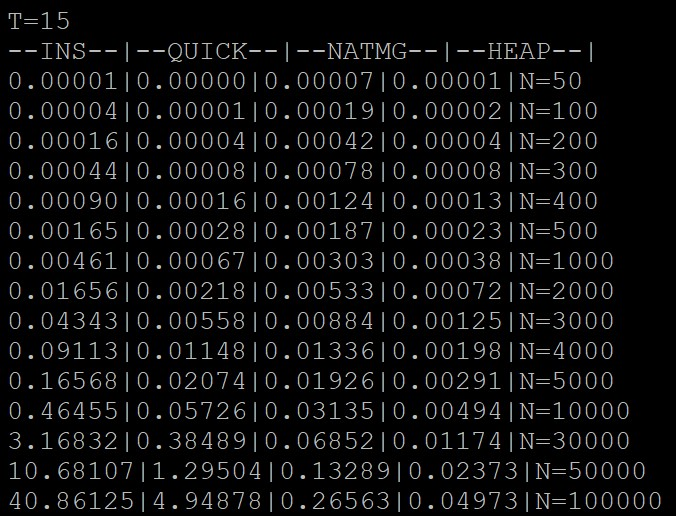
\includegraphics[width=0.48\textwidth]{result_decreasing.jpg}
        \label{fig:result_decreasing}
    }
    \subfigure[Sorted result]{
        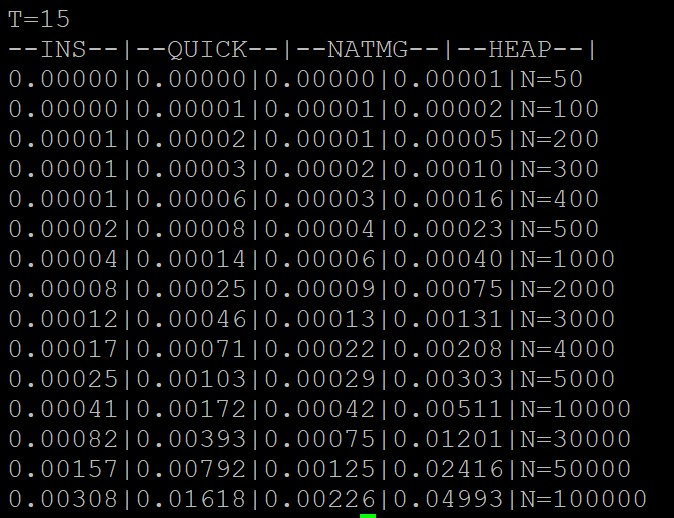
\includegraphics[width=0.48\textwidth]{result_sorted.jpg}
        \label{fig:result_sorted}
    }
    \subfigure[Partially sorted result]{
        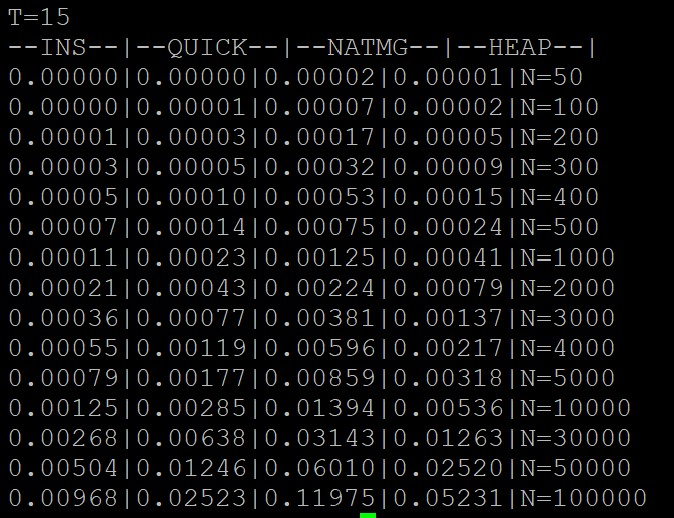
\includegraphics[width=0.48\textwidth]{result_partially_sorted.jpg}
        \label{fig:result_partially_sorted}
    }
    \subfigure[Random result]{
        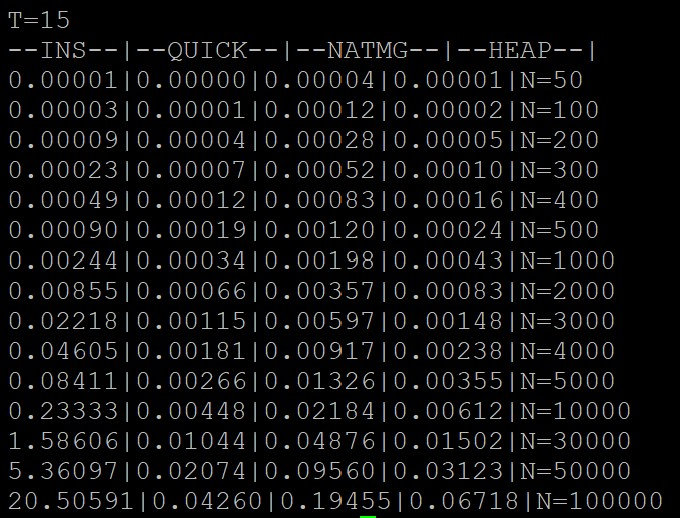
\includegraphics[width=0.48\textwidth]{result_random.jpg}
        \label{fig:result_random}
    }
    \caption{결과}
    \label{fig:result}
\end{figure}

\begin{figure}
    \centering
    \subfigure[Decreasing result]{
        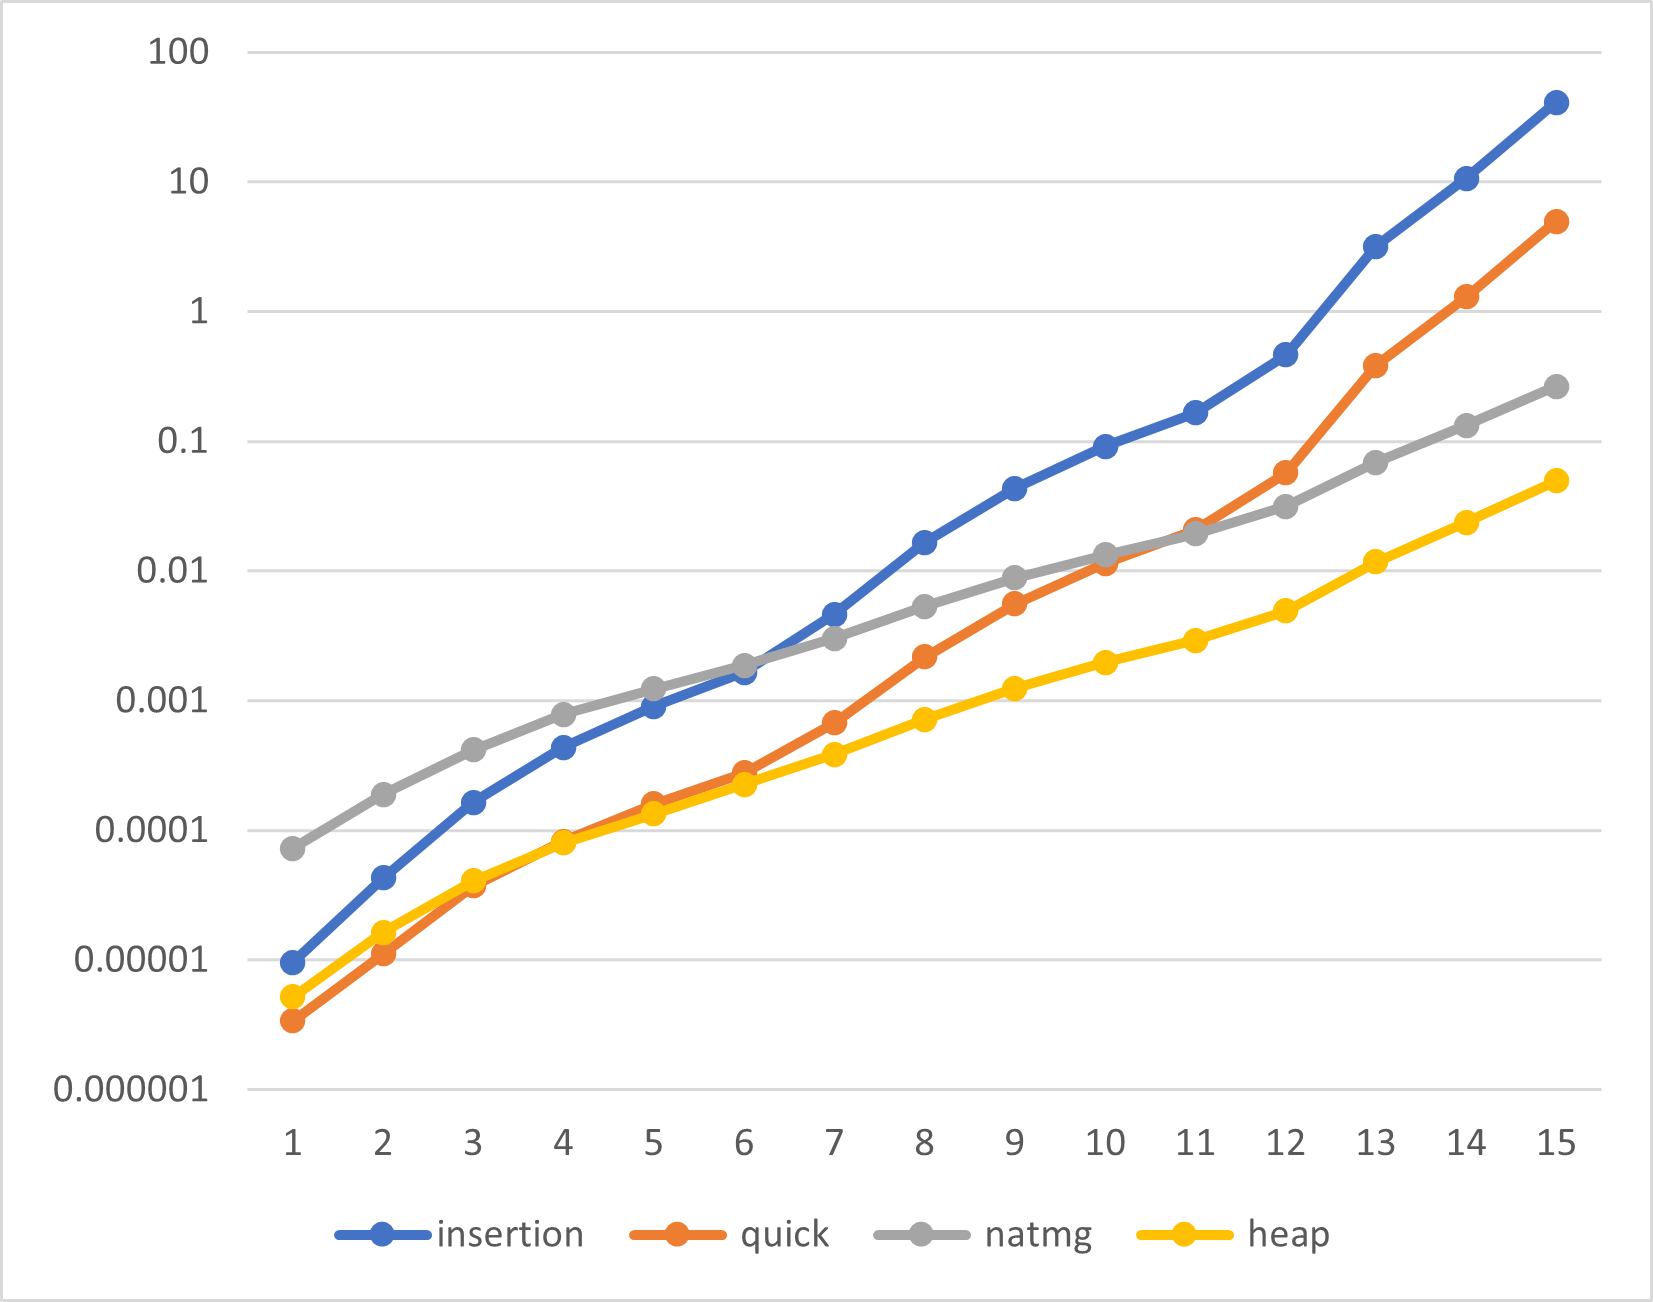
\includegraphics[width=0.48\textwidth]{resultchart_decreasing.png}
        \label{fig:result_decreasing_chart}
    }
    \subfigure[Sorted result]{
        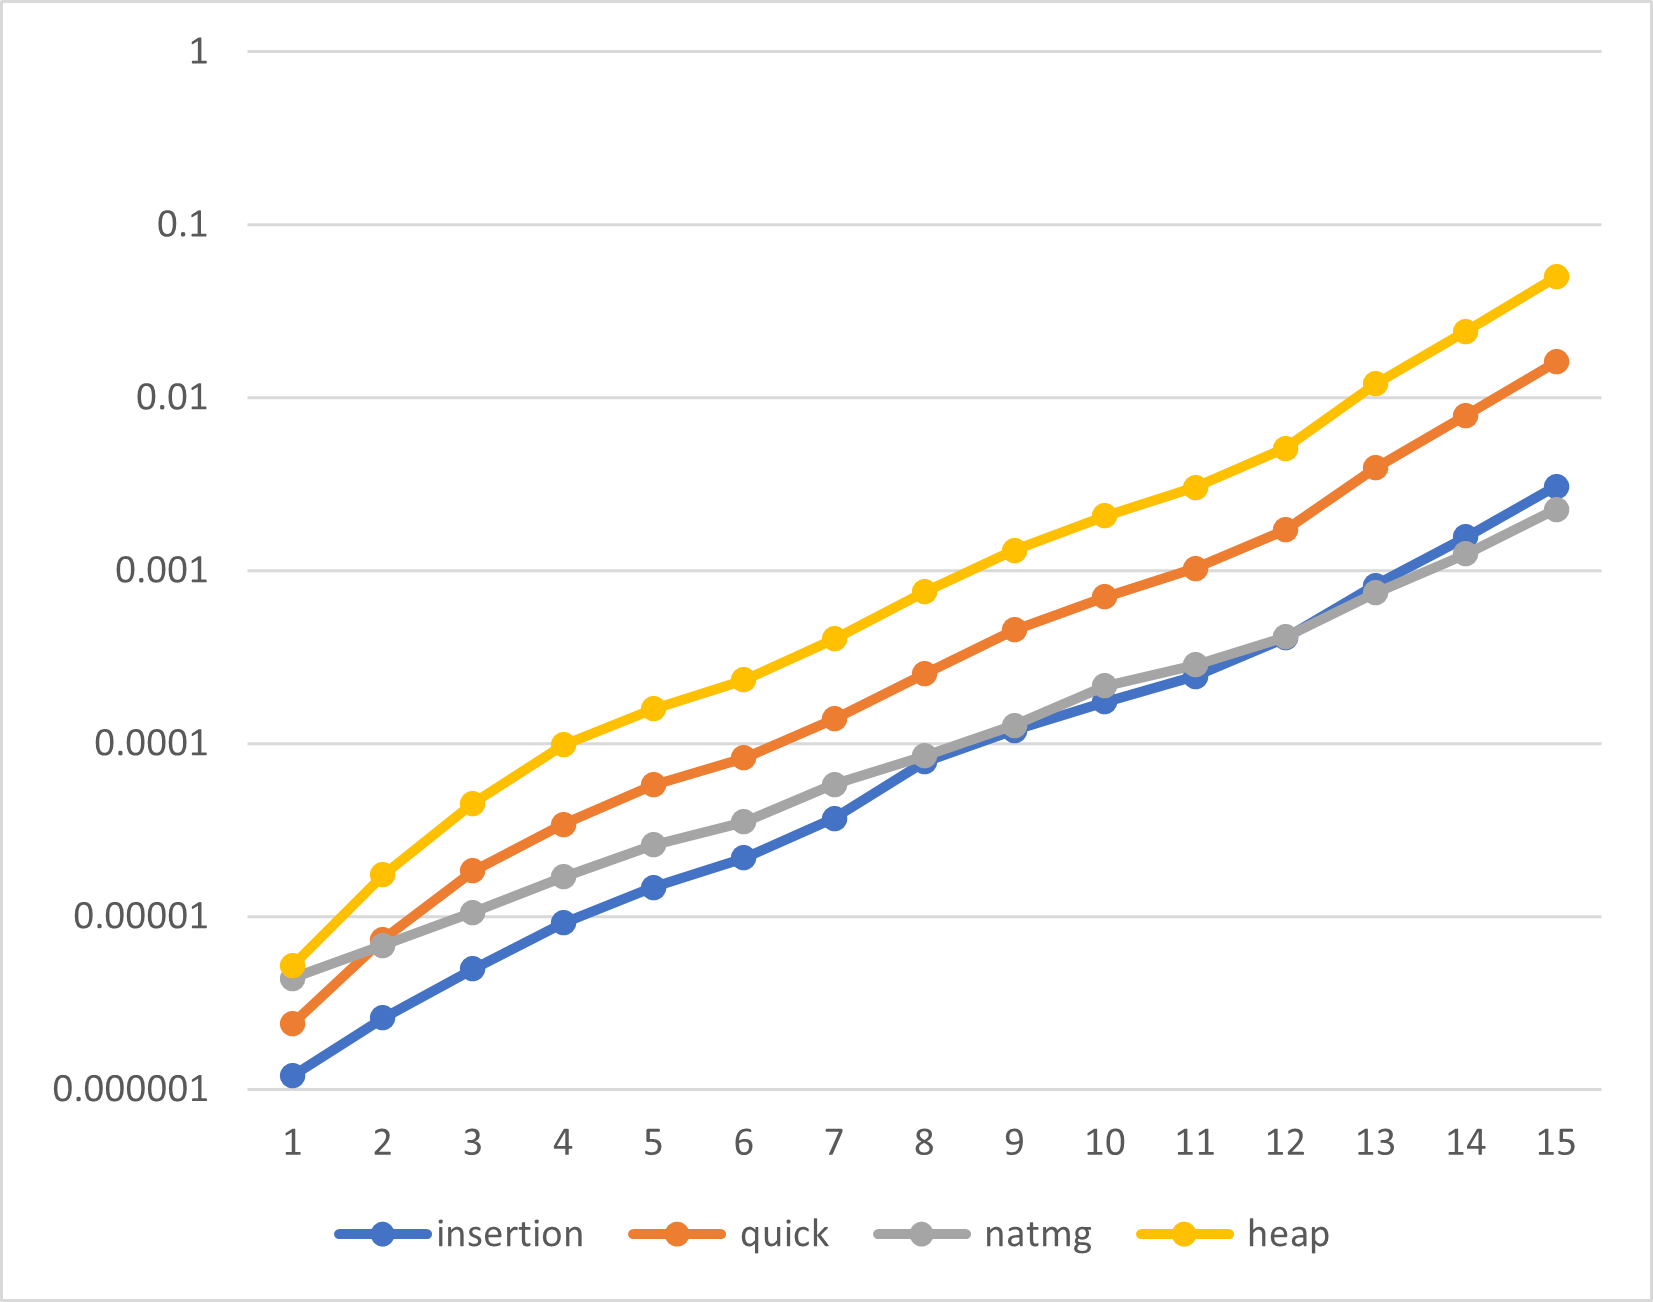
\includegraphics[width=0.48\textwidth]{resultchart_sorted.png}
        \label{fig:result_sorted_chart}
    }
    \subfigure[Partially sorted result]{
        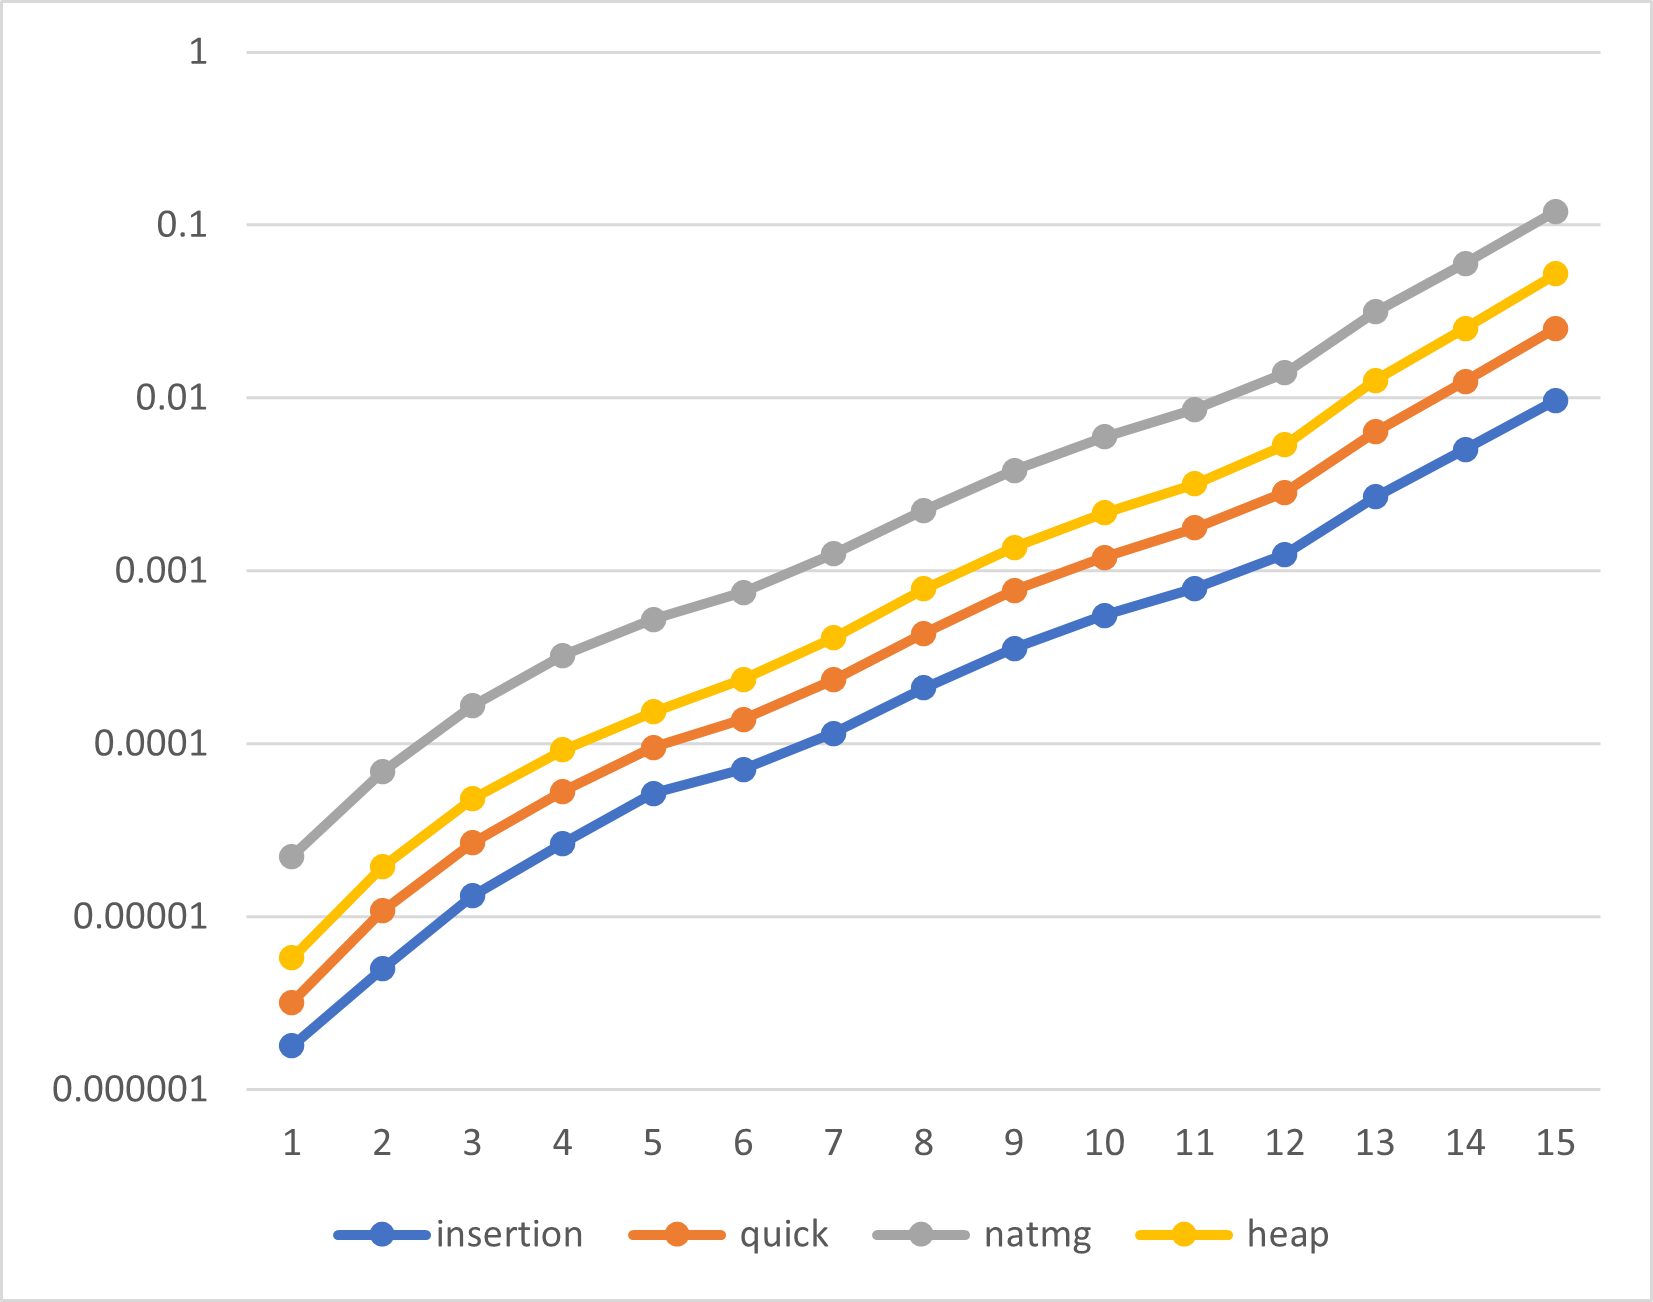
\includegraphics[width=0.48\textwidth]{resultchart_partially_sorted.png}
        \label{fig:result_partial_chart}
    }
    \subfigure[Random result]{
        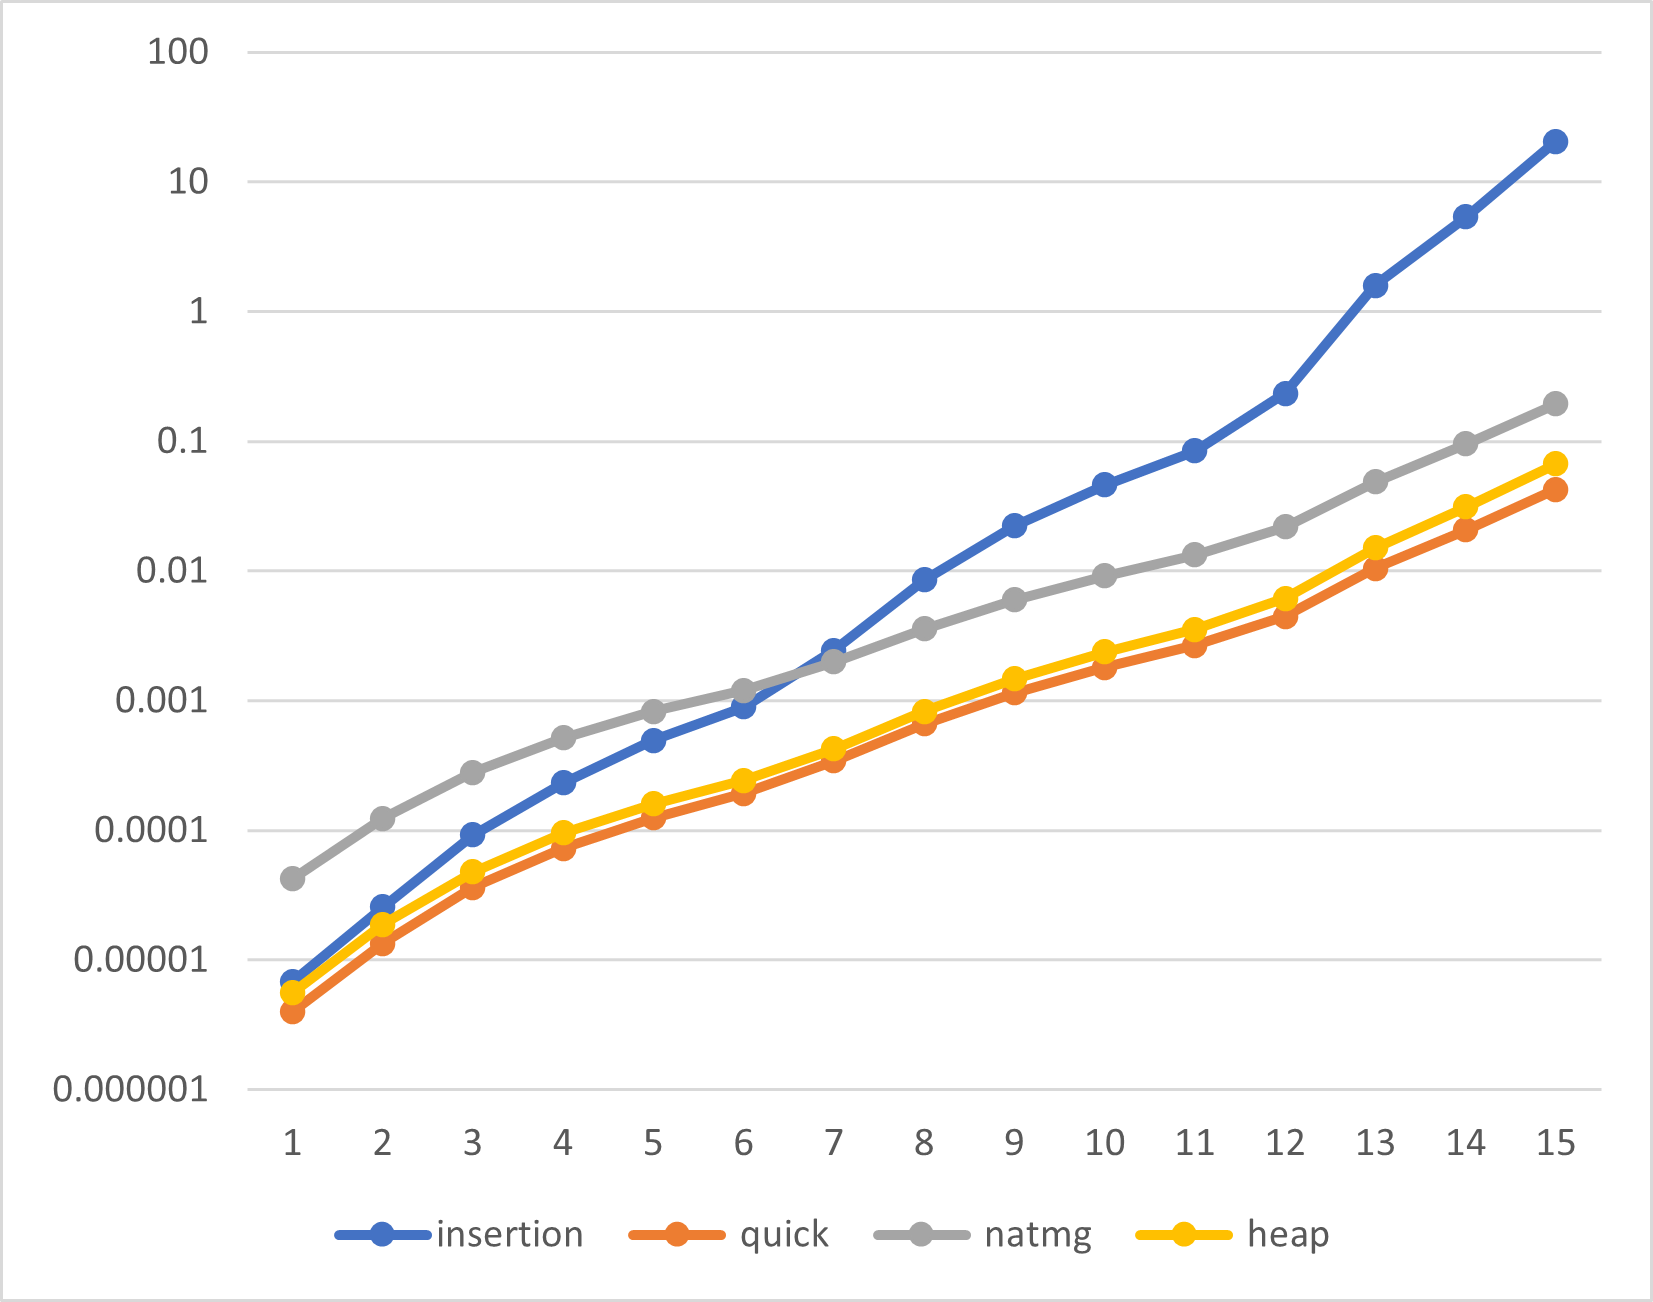
\includegraphics[width=0.48\textwidth]{resultchart_random.png}
        \label{fig:result_random_chart}
    }
    \caption{결과 차트}
    \label{fig:result_chart}
\end{figure}

알고리즘 성능 분석 환경은 linux 환경에서 진행하였다. 그림 \ref{fig:result_chart}에 앞선 결과의 차트 그림이 나와 있다. 자세한 수치는 그림 \ref{fig:result}에서 확인할 수 있다. 그림 \ref{fig:result_chart}은 \underline{\textit{로그 스케일}}임에 주의하라. 눈금 한 칸 당 10배 씩 차이난다. x축의 1, 2, $\cdots$, 15는 각각 t50.txt, t100.txt, $\cdots$, t100000.txt 파일에 대응한다. 성능은 걸린 시간이 빠를 수록, 즉 y축에서 아래에 있을 수록 좋다.
각 상황에 대해 살펴보자.
\begin{itemize}
    \item Decreasing의 경우(그림 \ref{fig:result_decreasing}, \ref{fig:result_decreasing_chart}): 최악의 경우의 시간 복잡도이다. 특히 삽입 정렬의 경우 데이터의 수가 늘어날 수록 연산 시간은 기하 급수적으로 증가해, 데이터 100,000개를 정렬할 때 평균 40.9초의 시간이 소요되었음을 알 수 있다. 한편 퀵 정렬을 주목한다면, 최악의 경우 퀵 정렬은 힙 정렬이나 자연 합병 정렬보다 훨씬 안 좋은 성능을 보여주었다. 한편 데이터의 수가 적을 때(그림 \ref{fig:result_decreasing_chart}에서 400개보다 작을 때를 주목한다면) 삽입 정렬이 자연 합병 정렬보다 더 좋은 성능을 보여주었다.
    \item Sorted의 경우(그림 \ref{fig:result_sorted}, \ref{fig:result_sorted_chart}): 최선의 경우의 시간 복잡도이다. 특히 데이터의 수가 2000개일 때까지도 삽입 정렬이 제일 우수한 성능을 보여주었다. 데이터의 수가 그보다 많을 때에도 삽입 정렬은 퀵, 힙 정렬보다 더 우수한 성능을 보여주었다. 이는 삽입 정렬 특성상 이미 정렬된 데이터에 대해서는 고려하지 않고 넘어가기 때문이며, 마찬가지 이유로 이미 정렬된 서브 리스트를 고려하는 자연 합병 정렬 역시 정렬된 데이터가 많을 수록 성능 면에서 유리하다.
    \item Partially sorted의 경우(그림 \ref{fig:result_partially_sorted}, \ref{fig:result_partial_chart}): 부분 정렬된 경우이다. 이 경우 모든 데이터의 경우에 대해 삽입 정렬이 가장 우수한 성능을 보여주었다.
    \item Random의 경우(그림 \ref{fig:result_random}, \ref{fig:result_random_chart}): 일반적인 상황에서 가장 많이 보게 될 경우이다. 삽입 정렬의 경우 데이터의 수가 적을 때는 자연 합병 정렬보다 더 우수했으나 500개 즈음에서 교차되어 이후부턴 기하 급수적으로 연산 시간이 늘어났다. 다른 세 정렬 중 퀵 정렬이 가장 우수한 성능을 보여주었음을 알 수 있다.
\end{itemize}
아쉬운 점은 자연 합병 정렬이 비휴율적으로 구현하여 최적의 성능을 발휘하지 못하는 것으로 추정된다. Vector, pair 클래스가 매우 무거운 클래스인 탓에, 이를 계속 생성하고 해제하는 과정에서 큰 성능 저하가 일어난 것으로 보인다. 자연 합병 정렬에 더 좋은 아이디어를 도입해서 최적화시킬 필요가 있어보인다.

\subsection{피벗 선택 방식에 따른 퀵 정렬 성능 비교}
Decreasing의 경우 퀵 정렬이 자연 합병 정렬이나 힙 정렬에 비해 크게 뒤쳐진다는 것을 알 수 있다. 그러나 이는 나름의 피벗 선택 과정에 있어서 중앙값을 선택하는 개선된 버전을 사용하였기에 선방한 결과이다. 만약 피벗을 단순히 서브 리스트의 맨 왼쪽 요소로 선택할 경우, 어떻게 될까? 두 경우에 대해 Decreasing 상황을 비교해보자\footnote{코드의 경우, 코드 \ref{lstlinsting:quick sort}에서 pivotIdx를 선택하고 이를 left와 스왑하는 두 줄의 코드를 삭제하여 구현하였다.}.

\begin{figure}
    \centering
    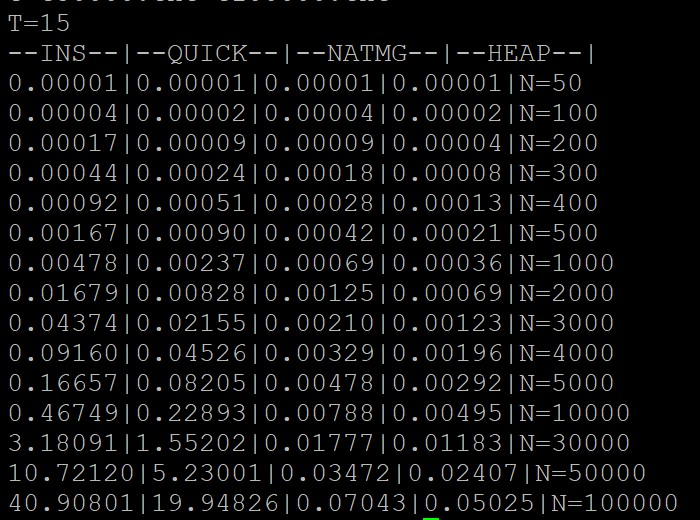
\includegraphics{result_quick_notMedian_decreasing.jpg}
    \caption{퀵 정렬에서 중앙값을 선택하지 않았을 경우 Decreasing 결과}
    \label{fig:not median result}
\end{figure}

\begin{figure}
    \centering
    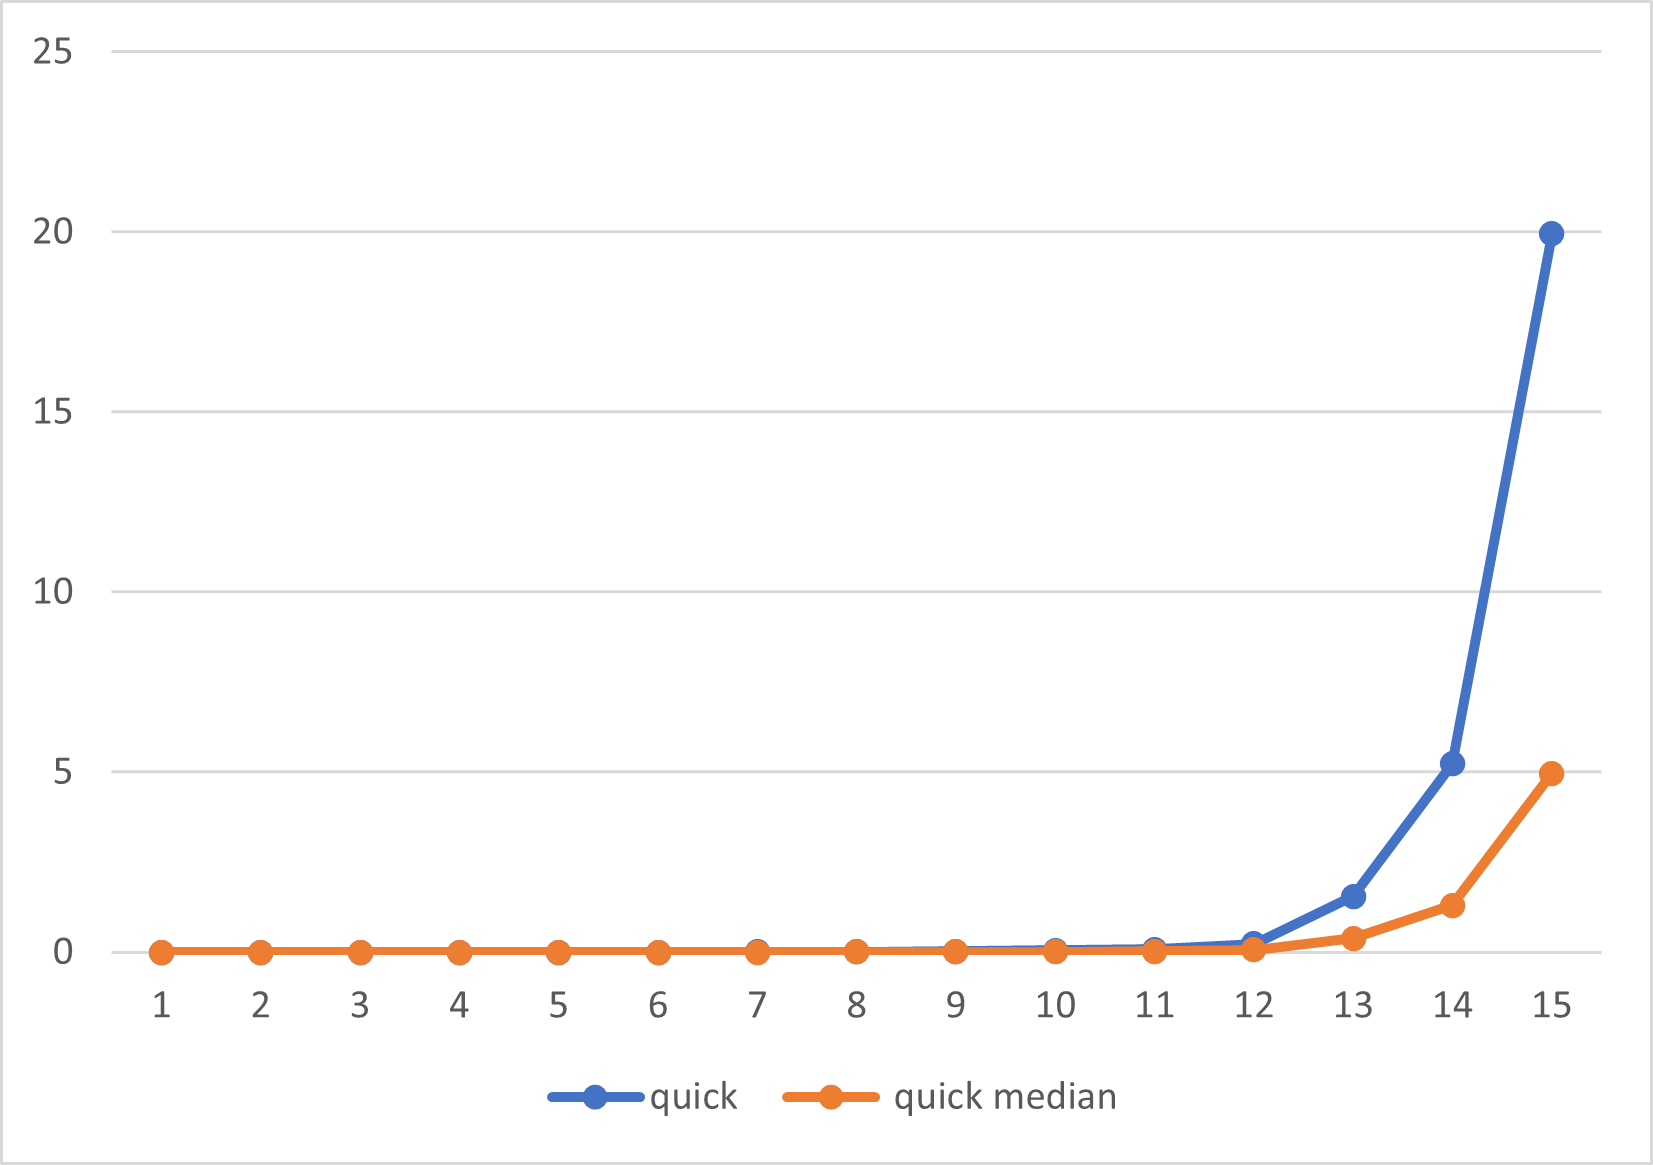
\includegraphics{compare_quick_pivot.png}
    \caption{피벗 선택 방식에 따른 퀵 정렬 성능 비교}
    \label{fig:compare quick with pivot}
\end{figure}

퀵 정렬에서 피벗을 단순히 서브 리스트의 맨 왼쪽으로만 선택했을 경우, Decreasing에 대한 결과는 그림 \ref{fig:not median result}과 같이 되며, 두 결과를 퀵 정렬에 대해서 비교해보면 그림 \ref{fig:compare quick with pivot}\footnote{이번엔 로그 스케일이 \underline{아님}에 주의하라.}와 같다. 데이터의 수가 적을 때에도 중앙값 방식이 우수하지만, 특히 데이터의 수가 많아질 경우 그 효과는 크게 증가하는 것을 확인할 수 있으며, 이는 최악의 경우 상황에 두드러진다.
\end{document}
